\documentclass[12pt]{article}
\usepackage[margin=1in]{geometry}
\usepackage{hyperref}
\usepackage{subcaption}
\usepackage{setspace}
\usepackage{graphicx}
\usepackage[toc,page]{appendix}
\usepackage{scrextend}
\usepackage{pgfplots}
\usepackage{listings}
\usepackage{natbib}
\usepackage[T1]{fontenc}
\usepackage[utf8]{inputenc}
\usepackage{lmodern}
\usepackage{subcaption}
\expandafter\def\csname ver@subfig.sty\endcsname{}
\usepackage{svg}
\usepackage{amssymb}
\usepackage{courier}

\setlength\parskip{5mm}
\widowpenalty10000
\clubpenalty10000
\setlength\parindent{0pt}

\lstset{ %
  language=C,
  directivestyle={\color{black}},
  emph={int,char,double,float,unsigned,struct},
  emphstyle={\color{blue}},
  backgroundcolor=\color{white},   % choose the background color; you must add \usepackage{color} or \usepackage{xcolor}
  breakatwhitespace=false,         % sets if automatic breaks should only happen at whitespace
  breaklines=true,                 % sets automatic line breaking
  captionpos=b,                    % sets the caption-position to bottom
  escapeinside=\`\`,               % if you want to add LaTeX within your code
  extendedchars=true,              % lets you use non-ASCII characters; for 8-bits encodings only, does not work with UTF-8
  frame=single,	                   % adds a frame around the code
  keepspaces=true,                 % keeps spaces in text, useful for keeping indentation of code (possibly needs columns=flexible)
  keywordstyle=\color{blue},       % keyword style
  numbers=left,                    % where to put the line-numbers; possible values are (none, left, right)
  numbersep=5pt,                   % how far the line-numbers are from the code
  rulecolor=\color{black},         % if not set, the frame-color may be changed on line-breaks within not-black text (e.g. comments (green here))
  showspaces=false,                % show spaces everywhere adding particular underscores; it overrides 'showstringspaces'
  showstringspaces=false,          % underline spaces within strings only
  showtabs=false,                  % show tabs within strings adding particular underscores
  stepnumber=2,                    % the step between two line-numbers. If it's 1, each line will be numbered
  tabsize=2,	                   % sets default tabsize to 2 spaces
  title=\lstname                   % show the filename of files included with \lstinputlisting; also try caption instead of title
}

\lstset{basicstyle=\ttfamily,breaklines=true}

\begin{document}
\begin{center}

	UNIVERSITY of CALIFORNIA\\
	\vspace{2mm}
	SANTA CRUZ\\
	\vspace{10mm}
	{\large\textbf{\textsc{SOLVING BOUNDARY VALUE PROBLEMS\\EFFICIENTLY USING COMPUTERS}}}\\
	\vspace{10mm}
	A thesis submitted in partial satisfaction\\of the requirements for the degree of\\
	\vspace{5mm}
	\textsc{BACHELOR OF SCIENCE}\\
	\vspace{3mm}
	in\\
	\vspace{3mm}
	\textsc{PHYSICS}\\
	\vspace{5mm}
	by\\
	\vspace{2mm}
	Daniel A. Bittman\\
	May 29, 2016\\

	\vspace{2in}

	The thesis of Daniel A. Bittman is approved by:\\
	\vspace{1in}

	\rule{2.5in}{2pt}\hfill
	\rule{2.5in}{2pt} \\
	Professor Jason Nielsen \hfill Professor David P. Belanger\\
	Thesis Adviser \hfill Thesis Coordinator\\

	\vspace{15mm}
	\rule{2.5in}{2pt}\\
	Professor Robert Johnson\\
	Chair, Department of Physics

\end{center}

\pagenumbering{gobble}
\clearpage
\setcounter{page}{1}
\renewcommand{\thepage}{\roman{page}}

\begin{center}
	\textsc{{\Large Copyright and Software License}}\\
	\vspace{1in}
	\textsc{this document and software described herein are\\\vspace{5mm}copyright} \copyright $\;$\textsc{2016\\daniel a. bittman}\\
	\vspace{1in}
	\textsc{The software described herein, including excerpts and other code, is provided with the following license:}

	MIT License

Copyright \copyright $\;$ 2016 Daniel A. Bittman

Permission is hereby granted, free of charge, to any person obtaining a copy
of this software and associated documentation files (the ``Software''), to deal
in the Software without restriction, including without limitation the rights
to use, copy, modify, merge, publish, distribute, sublicense, and/or sell
copies of the Software, and to permit persons to whom the Software is
furnished to do so, subject to the following conditions:

The above copyright notice and this permission notice shall be included in all
copies or substantial portions of the Software.

THE SOFTWARE IS PROVIDED ``AS IS'', WITHOUT WARRANTY OF ANY KIND, EXPRESS OR
IMPLIED, INCLUDING BUT NOT LIMITED TO THE WARRANTIES OF MERCHANTABILITY,
FITNESS FOR A PARTICULAR PURPOSE AND NONINFRINGEMENT. IN NO EVENT SHALL THE
AUTHORS OR COPYRIGHT HOLDERS BE LIABLE FOR ANY CLAIM, DAMAGES OR OTHER
LIABILITY, WHETHER IN AN ACTION OF CONTRACT, TORT OR OTHERWISE, ARISING FROM,
OUT OF OR IN CONNECTION WITH THE SOFTWARE OR THE USE OR OTHER DEALINGS IN THE
SOFTWARE.

\end{center}
\clearpage

\begin{addmargin}[8em]{8em}
\begin{center}

	\textbf{Dedication}
	\vspace{50mm}

	To my loving parents, Steve Bittman and Ellen Klima, for their unending support
	and unwavering belief in my ability to succeed.

	\vspace{100mm}
	Also for Frankie.
\end{center}

\begin{addmargin}[6.2em]{8em}
\begin{verbatim}
      \    /\
       )  ( ')
      (  /  )
       \(__)|
\end{verbatim}
\end{addmargin}
\end{addmargin}
\clearpage
\begin{center}
	\textbf{Acknowledgements}
	\vspace{50mm}

	A huge thank you to my thesis adviser, Jason Nielsen, for providing the opportunity
	to work on this interesting project, and for the many interesting conversations over
	the quarters past.

	\vspace{10mm}
	The Storage Systems Research Center at UC Santa Cruz for some of their machines in order
	to test the performance of this system.

\end{center}
\clearpage
\tableofcontents
\clearpage
\listoffigures
\listoftables
\clearpage
\renewcommand{\lstlistlistingname}{List of Source Code Listings}
\lstlistoflistings
\clearpage

\renewcommand{\thepage}{\arabic{page}}
\setcounter{page}{1}
\section*{Abstract}

\onehalfspacing

There are many problems in physics which involve solving a set of equations which define behavior
inside some region. One such set of problems, among many, is solving electrostatics problems inside
a region given some boundary conditions by utilizing Poisson's equation. Such problems, and other
problems, are commonly found in simple and analytically solvable forms in undergraduate physics classes.
Unfortunately, these problems can become intractable to solve analytically very quickly as their complexity
increases. Complex boundary conditions in strangely shaped regions can easy become impossibly difficult to
solve. The solution to this problem can be to model it on a computer in order to compute a numerical solution
in place of an analytical one.

I have written a software package which is both a C library which can solve such a given problem and a frontend
Python program which can parse a human-readable configuration that describes such a boundary value problem and
set up the correct initial state such that the C library can then solve it, allowing the Python program to
display the final result as well as calculate statistics about the solving process. I have utilized effective
programming techniques designed for current generation hardware 64-bit x86 processors in order to improve
the performance of the program, in addition to implementing a multi-threaded version of the solving program
to explore the use of multi-core processors in solving these problems.

I found that the program correctly matched an analytical solution to a simple test problem, and that it correctly
predicted the $1/r^2$ potential found from an electric dipole. I was able to optimize the program so that it
efficiently found these results, and I was able to successfully leverage multi-threading to significantly increase
the performance, albeit with a degradation in simulation accuracy.

\clearpage
\doublespacing
\section{Introduction}

Boundary value problems, problems defined by a partial differential equation and a set of
constraints on the solution, are found in many areas of physics. These include problems
such as finding the temperature of a rod that has a given temperature on either end,
determining the electric potential inside a region given the potential around the
boundary, or determining the flow of an incompressible fluid. As the complexity of 
these problems increases, however, the feasibility of solving them exactly by hand
quickly decreases. Instead, we have the option to solve them with iterative methods
using computers. These types of problems are well-suited for computers because
they are easily parallelizable, can be discreetized easily, and require a lot of repetitive calculation~\cite{parallel}. I have developed an
implementation of such a solver for electrostatics utilizing the 
parallelizability of the problem and designed it to be efficient by taking advantage 
of the design of modern CPUs.

Although many differential equations are typically used in boundary value problems,
I will limit the focus to the Poisson equation. Named after Siméon Denis Poisson, the Poisson equation
is used in a number of typical boundary value problems, including electrostatics.
In 2-dimensional Euclidean space it is\cite{boas},
$$\nabla^2 u = f,$$
where $f$ is a real-valued function inside the space and $u$ is the steady-state
solution for the potential in the space. The problems that we are considering are called boundary value problems
because their solutions are dependent both on the value of $f$, but also on the properties of the region and its boundaries.
Formally, the problems to solve are given with $f$ defined and with a region $\Omega$ which has defined boundaries
$\partial\Omega$. These boundary conditions, along with $f$, are the primary inputs to the program which determine
the solution it will give.

\subsection{Discreetizing Poisson's Equation}

Since we are solving these problems using a computer, we must transform the problem definition into one which a computer
can actually calculate. Computers do not do well with continuous functions and real numbers. The process of transforming
a problem or equation into one which a computer can handle is called discreetization.

\begin{figure}[htb]
	\centering
	\includesvg{grid}
	\caption{Visualization of grid, with indicies.}
\label{grid}
\end{figure}

Consider a grid of size $n$ by $n$ as in figure~\ref{grid}\footnote{In general, it is not difficult to allow a rectangular grid, but for simplicity
we will require the grid to be square.}, with values represented by $u_{i,j}$. We want to apply the Poisson equation to
this $u$ as follows:
$$\nabla^2 u = \frac{\partial^2 u}{\partial x^2} + \frac{\partial^2 u}{\partial x^2} = f,$$
however, $u$ is not continuous, so the partial derivative for $x$ becomes
$$\frac{\partial^2 u}{\partial x^2} \approx \frac{u_{i-1,j} - 2 u_{i,j} + u_{i+1,j}}{h^2},$$
at a grid point $(i,j)$, where $h = 1 / n$ is the width and height of a grid cell. The partial derivative for $y$ is similar, using $j$ instead of $i$.
This gives the full discrete Poisson equation as\cite{poisson-relax}\cite{myths},
$$\frac{u_{i-1,j} - 2 u_{i,j} + u_{i+1,j}}{h^2} + \frac{u_{i,j-1} - 2 u_{i,j} + u_{i,j+1}}{h^2} = f_{i,j}.$$

Since $u_{i,j}$ is what we are interested in, this is more useful after some rearranging:
$$h^2f_{i,j} = -4u_{i,j} + u_{i-1,j} + u_{i+1,j} + u_{i,j-1} + u_{i,j+1},$$
\begin{equation} \label{eq:poisson}
u_{i,j} = \frac{1}{4}(u_{i-1,j} + u_{i+1,j} + u_{i,j-1} + u_{i,j+1} - h^2f_{i,j}).
\end{equation}

It can be seen from the top equation that this is now a linear algebra problem, requiring a method of solving
$n^2$ dependent linear equations. This means that we can apply one of several standard iterative methods
for solving the problem. This is an excellent application of using a computer to solve numerically a problem
	which is difficult to solve analytically.


\subsection{Jacobi Iteration}
This method is perhaps the simplest method of doing an iterative solution to this linear algebra problem. The procedure
involves treating each equation as independent, and solving iteratively. This turns Equation~\ref{eq:poisson} into\cite{poisson-relax}
\begin{equation} \label{eq:jacobi}
u_{i,j}^{k+1} = \frac{1}{4}(u_{i-1,j}^{k} + u_{i+1,j}^{k} + u_{i,j-1}^{k} + u_{i,j+1}^{k} - h^2f_{i,j}),
\end{equation}
where $k$ is the iteration number. This is saying that to calculate $u$ everywhere, we must start with a guess for $u$,
and then iteratively solve each element in $u$, which depends on its four nearest neighbors. One immediate unfortunate
reality with Jacobi iteration presents itself: we must store a secondary copy of the entire grid because each calculation
of $u_{i,j}^{k+1}$ strictly requires values from the previous iteration. Since we iterate over the grid in order to solve
it, we cannot write the new value for the $k+1$ iteration into that element of $u$, since we would be overwriting a value
that is needed later. This unforunately but necessarily increases the space required by a factor of $n^2$.

The above equation does not yet include any consideration of boundary conditions. The primary functionality of supporting solving statics problems requires support for dealing with
Dirichlet boundary conditions. Dirichlet boundary conditions are defined such that the solution $\phi$ of a partial
differential equations in a region $\Omega$ has a value $\phi(\mathbf{r}) = y(\mathbf{r}) \; \forall \mathbf{r} \in \partial \Omega$.
For this case, this means that if a Dirichlet boundary value condition is specified for a particular grid cell $(x,y)$,
then its value is simply fixed to the value of the Dirichlet condition, and that cell does not need to be recalculated on
successive iterations.

Another consideration is that the grid is of finite size. This means that when calculating $u_{i=0,j}$, for example, we cannot
incorporate $u_{i-1,j}$ as Equation~\ref{eq:jacobi} would dictate. This is because that would try to get the $-1^{st}$ row the
the matrix $u$, which does not exist. A common method of dealing with this problem is to ``wrap around'' to the other side --
essentially considering the region $\Omega$ to the surface of a sphere, or to consider the space to be periodic. Because of
the nature of the problems that I will be considering, I have chosen to consider an implicit Dirichlet boundary condition
of zero everywhere outside of $\Omega$, thus effectively limiting the calculation to be inside the region while clamping any
values ``outside'' of $\Omega$ to zero. This is easy to implement and visualize as well: any value of $u_{i,j}$ for $i >= n$,
$i < 0$, $j >= n$, or $j < 0$ is simply zero, always.

\subsection{Successive Over-Relaxation}

An alternate approach of iteratively solving this problem numerically is called successive over-relaxation (or SOR), and
it has advantages over simple Jacobi iteration. It works by reusing previous calculations for the next iteration when
calculating a given cell. It transforms Equation~\ref{eq:jacobi} into,
\begin{equation} \label{eq:sor}
u_{i,j}^{k+1} = (1-\omega) + \frac{\omega}{4}\left(u_{i-1,j}^{k+1} + u_{i+1,j}^{k} + u_{i,j-1}^{k+1} + u_{i,j+1}^{k} - h^2 f_{i,j}\right),
\end{equation}
where $\omega$ is a tunable parameter called the \textit{over-relaxtion parameter}. For a square lattice, a value of
$$\omega = \frac{2}{1+\frac{\pi}{n}}$$
has the best rate of convergence\cite{poisson-relax}. There are two terms on the right-hand-side of equation~\ref{eq:sor} which refer to the
$k+1$ iteration. What this is doing is using the new values for the cells that have already been updated on this iteration
in order to speed up the convergence.


%TODO Determining when to halt











\subsection{Performance Considerations}
While operations on a grid of values are parallelizable, there is a limit to
the effectiveness of multi-threading the algorithm. Take, for example, an average
modern processor with 4 cores each with a 256KB cache and a shared cache of 8MB\@. Each core
can only operate on a grid of 256 by 256 32-bit values before exhausting its cache.
A performance drop will occur if the grid size per core exceeds the core's cache
size. For example, should the grid size exceed 1440 by 1440 32-bit values,
the shared 8MB cache will
be filled, resulting in a massive performance penalty. For this reason, na\"{i}vely splitting
the grid into 4 areas and multi-threading the iteration may result in sub-par performance.

There are many other aspects of processor design that come into play when writing a program
such as this. Multithreaded synchronization aside, there are many details of caching that
need to be considered. Of course, optimizing a program is just like any experiment in that
it is absolutely vital to apply normal scientific practices when doing such work. Many make
the mistake of simply writing what they believe to be a more optimized version of a program
without measuring the resulting performance and comparing it to the previous version.

I would expect to see the performance enhanced by the use of multithreading, but insignificantly
due to the large amount of memory accesses made by the program throughout solving a given problem.



\section{Methods}

Ultimately, the heavy lifting in solving a potential problem involves solving a partial
differential equation -- in this case, Poisson's equation. Here we will be considering
the 2-dimensional Poisson equation in Euclidean space,
$$\nabla^2 \phi = f,$$
where $f$ is a real-valued function inside the space and $\phi$ is the steady-state
solution for the potential in the space. However, since this solution will be calcuated
numerically on a computer, we must discretize the equation so that it can be used to
represent a solution on a 2-dimensional grid.

\subsection{Discreetizing Poisson's Equation}

Consider a grid of size $n$ by $n$\footnote{In general, it is not difficult to allow a rectangular grid, but for simplicity
we will require the grid to be square.}, with values represented by $u_{i,j}$. We want to apply the Poisson equation to
this $u$ as follows:
$$\nabla^2 u = \frac{\partial^2 u}{\partial x^2} + \frac{\partial^2 u}{\partial x^2} = f,$$
however, $u$ is not continuous, so the partial derivative for $x$ becomes
$$\frac{\partial^2 u}{\partial x^2} \approx \frac{u_{i-1,j} - 2 u_{i,j} + u_{i+1,j}}{h^2},$$
at a grid point $(i,j)$, where $h = 1 / n$ is the width and height of a grid cell. The partial derivative for $y$ is similar, using $j$ instead of $i$.
This gives the full discrete Poisson equation as,
$$\frac{u_{i-1,j} - 2 u_{i,j} + u_{i+1,j}}{h^2} + \frac{u_{i,j-1} - 2 u_{i,j} + u_{i,j+1}}{h^2} = f_{i,j}.$$

Since $u_{i,j}$ is what we are interested in, this is more useful after some rearranging:
$$h^2f_{i,j} = -4u_{i,j} + u_{i-1,j} + u_{i+1,j} + u_{i,j-1} + u_{i,j+1},$$
\begin{equation} \label{eq:poisson}
u_{i,j} = \frac{1}{4}(u_{i-1,j} + u_{i+1,j} + u_{i,j-1} + u_{i,j+1} - h^2f_{i,j}).
\end{equation}

It can be seen from the top equation that this is now a linear algebra problem, requiring a method of solving
$n^2$ dependent linear equations.

\subsection{Iterative Methods}

Since we are using a computer, an iterative method is feasible to be used as a numerical solution method. In this
program, I have implemented two methods for solving these problems: Jacobi iteration, and successive over-relaxation (SOR).

\subsubsection{Jacobi Iteration}
This method is perhaps the simplest method of doing an iterative solution to this linear algebra problem. The procedure
involves treating each equation as independent, and solving iteratively. This turns Equation~\ref{eq:poisson} into
\begin{equation} \label{eq:jacobi}
u_{i,j}^{k+1} = \frac{1}{4}(u_{i-1,j}^{k} + u_{i+1,j}^{k} + u_{i,j-1}^{k} + u_{i,j+1}^{k} - h^2f_{i,j}),
\end{equation}
where $k$ is the iteration number. This is saying that to calculate $u$ everywhere, we must start with a guess for $u$,
and then iteratively solve each element in $u$, which depends on its four nearest neighbors. One immediate unfortunate
reality with Jacobi iteration presents itself: we must store a secondary copy of the entire grid because each calculation
of $u_{i,j}^{k+1}$ strictly requires values from the previous iteration. Since we iterate over the grid in order to solve
it, we cannot write the new value for the $k+1$ iteration into that element of $u$, since we would be overwriting a value
that is needed later. This unforunately but necessarily increases the space required by a factor of $n^2$.

%TODO: convergence condition?

The above equation does not yet include any consideration of boundary conditions. In fact, this is only valid for a region
that is unbounded. The primary functionality of supporting solving statics problems requires support for dealing with
Dirichlet boundary conditions. Dirichlet boundary conditions are defined such that the solution $\phi$ of a partial
differential equations in a region $\Omega$ has a value $\phi(\mathbf{r}) = y(\mathbf{r}) \; \forall \mathbf{r} \in \partial \Omega$.
For this case, this means that if a Dirichlet boundary value condition is specified for a particular grid cell $(x,y)$,
then its value is simply fixed to the value of the Dirichlet condition, and that cell does not need to be recalculated on
successive iterations.

Another consideration is that the grid is of finite size. This means that when calculating $u_{i=0,j}$, for example, we cannot
incorporate $u{i-1,j}$ as Equation~\ref{eq:jacobi} would dictate. This is because that would try to get the $-1$st row the
the matrix $u$, which does not exist. A common method of dealing with this problem is ``wrap around '' to the other side --
essentially considering the region $\Omega$ to the surface of a sphere, or to consider the space to be periodic. Because of
the nature of the problems that I will be considering, I have chosen to consider an implicit Dirichlet boundary condition
of zero everywhere outside of $\Omega$, thus effectively limiting the calculation to be inside the region while clamping any
values ``outside'' of $\Omega$ to zero. This is easy to implement and visualize as well: any value of $u_{i,j}$ for $i >= n$,
$i < 0$, $j >= n$, or $j < 0$ is simply zero, always.

\subsubsection{Successive Over-Relaxation}

An alternate approach to iteratively solving this problem numerically is called successive over-relaxation (or SOR), and
it has advantages over simple Jacobi iteration. It works by reusing previous calculations for the next iteration when
calculating a given cell. It transforms Equation~\ref{eq:jacobi} into,
\begin{equation} \label{eq:sor}
u_{i,j}^{k+1} = (1-\omega) + \frac{\omega}{4}\left(u_{i-1,j}^{k+1} + u_{i+1,j}^{k} + u_{i,j-1}^{k+1} + u_{i,j+1}^{k} - h^2 f_{i,j}\right),
\end{equation}
where $\omega$ is a tunable parameter called the \textit{over-relaxtion parameter}. For a square lattice, a value of
$$\omega = \frac{2}{1+\frac{\pi}{n}}$$
has the best rate of convergence. There are two terms on the right-hand-side of equation~\ref{eq:sor} which refer to the
$k+1$ iteration. What this is doing is using the new values for the cells that have already been updated on this iteration
in order to speed up the convergence.


TODO Determining when to halt


\subsection{Design of Solver}
The solving program is written in C in order to leverage the full performance of modern computers and is implemented
as a shared library (on \textsc{unix}) such that it can be linked with another program which sets up the initial conditions
before calling the solving function. The C code that does the solving is hereby refered to as the engine, while any code
that interfaces with the engine and provides a usable user interface is referred to as the frontend.

I have written an example frontend in Python, which is capable to parsing a configuration file which describes the
values of $f$, the initial boundary conditions, the grid size, and a number of other details about a given desired
setup (hereby collectively reffered to as a configuration). I have written several example configurations which I have used to
confirm the correctness of the solving program. For a more detailed technical description of the implementation, see Appendix~\ref{app:des}.

\subsection{Configurations and Mapping to Electrostatics}

TODO also talk about how the configuration is written (include advance features like circles)

\subsection{Verifying Correctness}

The clearest way to verify that the solver is working correctly is to test it out on a number of different configurations
for which the correct solution is known. My first choice here was a simple electrostatics problem straight out of a textbook:
%%TODO cite...

\begin{addmargin}[2em]{2em}% 1em left, 2em right
	Consider a square region with the bottom left corner at the origin with each side of length $L$. Let the potential
	along each side of the region be fixed at 0, except for the bottom side, which has a potential $V(x) = V_0 \sin(x \pi / L)$.
	What is the potential $V$ inside the region?
\end{addmargin}

This problem describes solving Laplace's equation (which is Poisson's equation with $f=0$), given some initial boundary conditions.
It can be solved analytically using a standard separation of variables trick. Assume
$$\phi = X(x) Y(y),$$
then
$$X''(x)/X(x) = -Y''(y)/Y(y) = -\lambda,$$
and by applying the boundary conditions, one comes to the solution
$$V(x,y) = \frac{\sinh(y \pi / L)}{\sinh(\pi / L)} \sin(x \pi / L).$$

In order to compare the result of my program with the analytical solution, I added a feature to the Python frontend
to accept a pre-made file containing a precalculated grid of the correct output by using the analytic solution. The
frontend then reads this file and compares it to the result of the solver.
%TODO: measurement of correctness.

\subsection{Potential From Electric Dipole}
Another correctness check is a simulation of an electric dipole. The potential from an electric dipole is well understood.
If two equal and opposite charges are separated on an axis by distance $d$, then at a point $p$ far away, the
potential is,
$$V = C\left(\frac{1}{r_0} - \frac{1}{r_1}\right),$$
where $r_0$ and $r_1$ are the distances from each charge, and $C$ is a constant. With some rearranging,
$$V = C\left(\frac{r_0 - r_1}{r_0 r_1}\right) = \frac{C d \cos(\theta)}{r^2},$$
where $r$ is the distance from the center of charge to the point, and $\theta$ is the angle that the line from the
center of charge forms with the axis that the dipole is on. The potential from an electric dipole falls off as $1/r^2$,
which should be reflected in the solution given by the program if it is given a configuration describing a dipole.

If the solving program is correct, then if two charges are placed near each other, the numerically calculated potential
should display this $1/r^2$ behavior. I wrote such a configuration and had the frontend output the potential at points
increasing in distance from the center of the dipole, allowing me to fit the data to a $1/r^2$ curve.


Correctness Checks
 - Solution to sin(x) along wall potential -- non-discreet.
 - Electric dipole solution for far away

Calculating correctness automatically

\subsection{Optimization and Multithreading}
The purpose of this program is to not only be correct, but to be correct quickly. In order to achieve this, I have
tried three things in combination:
\begin{enumerate}
\item General program optimization, targeted towards 64-bit x86 machines
\item The use of the x86 SIMD instruction set
\item The use of multithreading to split up the work among CPU cores
\end{enumerate}
The first of these is pretty basic. The main part of the solver is written in C so that it can run directly on the
processor. When the program is compiled, I instruct the compiler to optimize the program to the best of its ability,
and the program is written in such a way that it can be optimized well and does not waste time doing unneccesary work.

As an example of the last point, consider a 2-dimensional grid (2-D array), which must be iterated over (much like
this program does). There are two ways to do this: either iterate row-by-row, or column-by-column. The end result is
the same, and one might think the choice is arbitrary. However, when I tested the two different approaches, I found
the row-by-row approach to be around 5 times faster. This is because of caching effects and the way that the CPU
fetches data from RAM. For a more detailed description of this, see Appendix~\ref{app:opt}.

Another example involves data structure organization. Say a program needs to store an array of objects, and each object
has data associated with it (for example, current value, previous value, error, initial state, etc). One might be tempted
to write something like in Listing~\ref{lst:aos}. The problem here is that if each object's \textsc{cur\_val} are all
calculated together (as is often the case, and is definitely the case for this solving program), then the location of
the values that need to be loaded in succession by the processor are far apart. This, again, comes down to caching
effects which are further explained in Appendix~\ref{app:opt}.

\begin{minipage}{\linewidth}
\begin{lstlisting}[frame=single,label=lst:aos,caption={Array of structures organization.}]
struct {
	double cur_val, prev_val;
	float err;
	int initial_state;
} objects[N];
\end{lstlisting}
\end{minipage}

Fortunately, this also has an easy to make change that drastically improves performance: change to structure of
arrays organization, thus reorganizing the memory layout so that related and commonly accessed-together values
appear adjacent in memory. This is shown in listing~\ref{lst:soa}. While it may be a less intuitive way to describe
and program a simulation, the result is significantly faster code the majority of the time.

\begin{minipage}{\linewidth}
\begin{lstlisting}[frame=single,label=lst:soa,caption={Structure of arrays organization.}]
struct {
	double cur_val[N];
	double prev_val[N];
	float err[N];
	int initial_state[N];
} objects;
\end{lstlisting}
\end{minipage}

\subsection{SIMD Instructions}
I have also made use of the SIMD (Single Instruction Multiple Data) instruction set. These instructions are available
on modern 64-bit x86 processors\footnote{More instructions are added in most new releases of CPUs. There are different
SIMD instruction sets available on different processor models. I have used the sse through avx instruction sets in this
code.}. Their purpose is to enable whats known as vector processing of data on x86 machines. This provides the ability
to apply a mathematical operation to one or more arrays, and have that operation by applied to each element. For example,
I can have a 128-bit register filled with 4 values, $x=(1,2,3,4)$, and other register like it, $y=(10, 10, 11, 11)$. I can
then add them together to get $(11, 12, 14, 15)$, and this addition is issued with a single instruction. Furthermore, this
takes the same amount of time as a single addition, because the processor can do the 4 separate addition operations in
parallel.

I have written in the use of SIMD instructions in the solver program in order to both reduce branches and to parallelize
the calculations required when calculating the next iteration of a given cell. I provided the ability to disable this
functionality and instead do a non-SIMD style calculation in order to get benchmarks. A requirement of the SIMD code was
that it give exactly the same result as the non-SIMD version (otherwise the implementation of the math would be incorrect).
For this reason, when talking about the results of a simulation, it does not matter if SIMD was used or not; the use
of SIMD only affects performance.

An important note is that when fully optimizing code for a machine which it knows about, \texttt{gcc} may choose to output
SIMD instructions in order to do computation even if the user does not do so explicitly. For this reason, in places where
I refer to the mode of the simulation as being ``non-SIMD'', what I mean is that it does not use my manual SIMD instructions
but it may still use compiler-generated SIMD instructions.

\subsection{Multithreading}
Finally, I have added multithreading support to the solver. This is done by spitting up the grid into subregions which
are contiguous in memory, and spawning $N$ threads via the pthreads API. Each thread is then given a region to work on,
and they coordinate through shared state in order to decide when the solution has been reached. The initial implementation
showed extremely poor results with multithreading (often being drastically slowed than the single threaded version)
due to the use of atomic shared variables. It was then re-written such that the code was unsafe but much faster. This
is because each thread modifies a shared non-atomic variable that keeps track of the current total change per iteration
after that thread itself completes a number of iterations over its region. This kind of shared memory access is much faster
than coordinating the threads, but it is also technically undefined behavior in C. Fortunately, on x86, it is actually
safe, however there is potential information loss because a thread could overwrite another thread if they are trying to
update the value at the same time. A more detailed discussion of the code and why it is unsafe can be found in Appendix~\ref{app:opt}.

\subsection{Benchmarking Performance}
Benchmarks were done by placing two calls to \texttt{gettimeofday(3)} around the core of the solver. This function has a
granularity of 1 microsecond CITE ME. This code returns
both the number of iterations done and the difference between the two gettimeofday calls, which are then used to calculate
the iterations per second. In order to take into account error from unpredicatble scheduling effect from the operating system,
each benchmark was run 300 times, and the standard deviation and mean were calculated, along with 95\% confidence intervals. Several different computers were used:
computer A was an Intel Core i5-3570K with 4 cores running at 3.4GHz with 16GB of RAM. Computer B was an Intel Xeon E5620
with 4 cores with 2 threads each, running at 2.4GHz, with 24GB of RAM. Computer B did not support all of the SIMD instructions
that I used, so it was only able to benchmark the non-SIMD version of the code.



\section{Results}

All results describing the correctness of the simulation or discussing the closeness of the simulation to an analytical
result are done using the single-threaded mode. This is because this makes the result of the simulation deterministic,
and so it does not matter which machine the test was run on. For results that measure performance, the machine and options
for the simulation used will be specified. There are times when the number of threads affected the correctness of the
result.

\subsection{The $\sin(x)$ Potential}

	\begin{figure}[h]
	\centering
	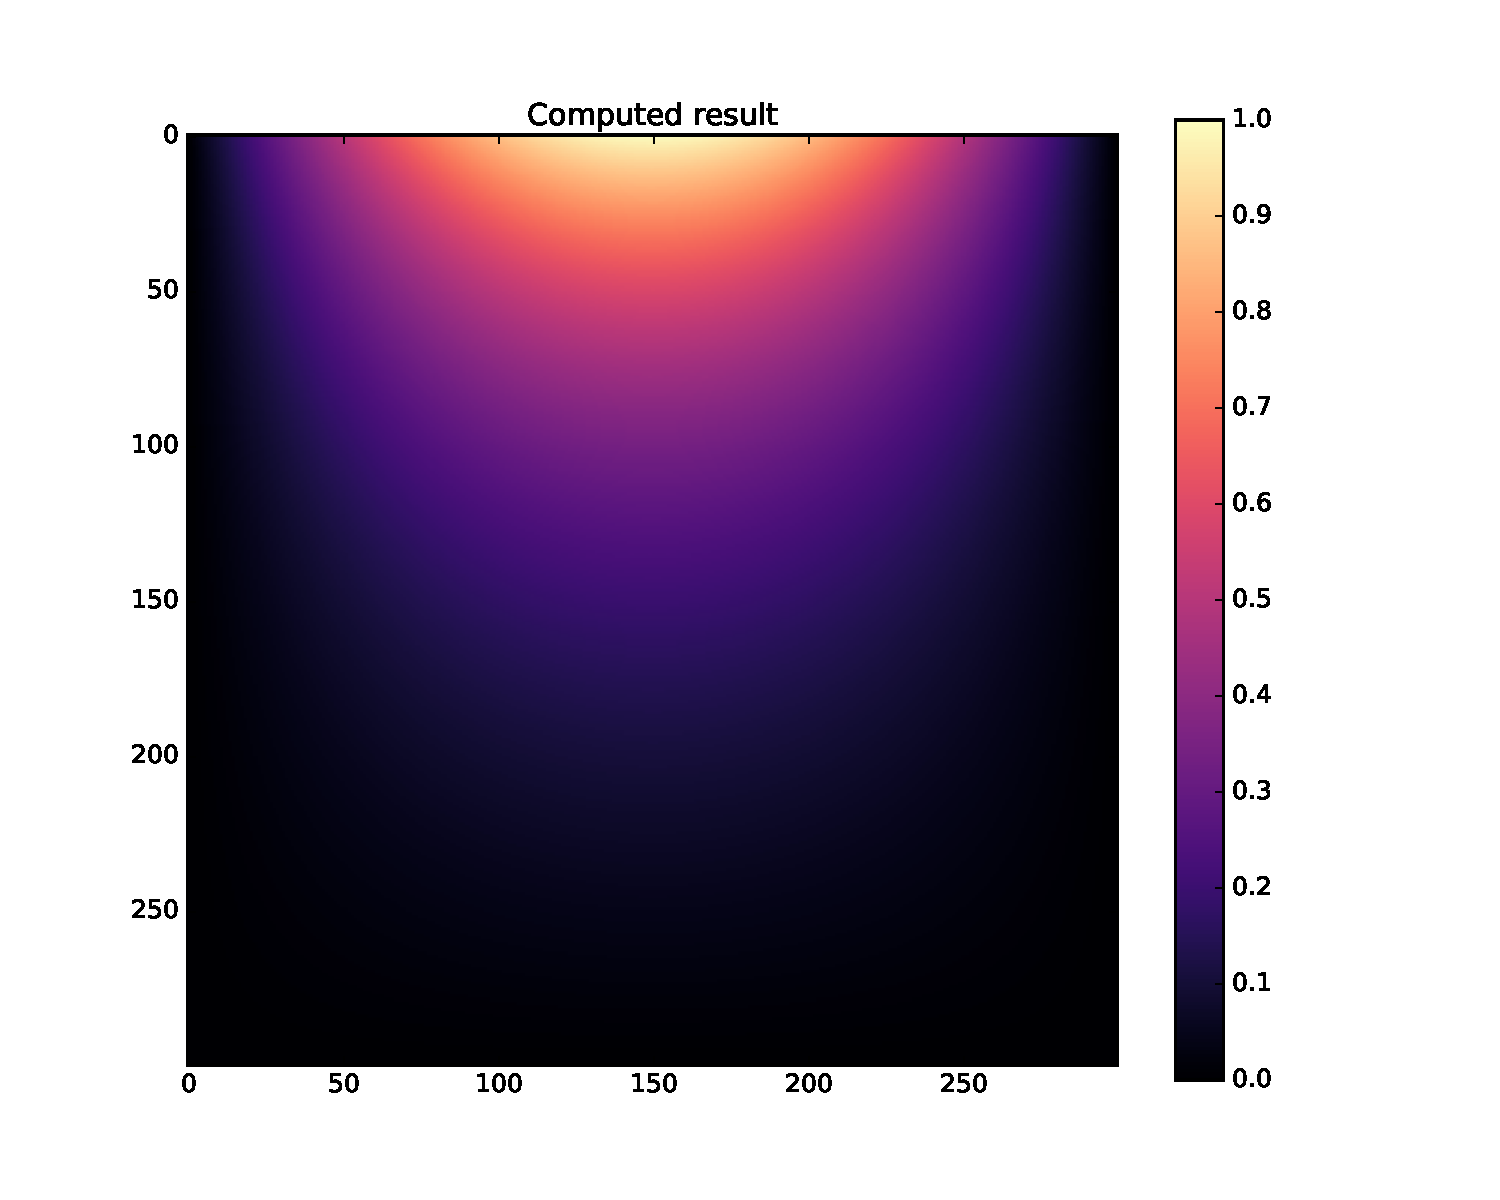
\includegraphics[width=1.1\linewidth]{sin300_calc.pdf}
	\caption{Simplistic view of CPU and RAM.} 
	\label{fig:sin-result}
	\end{figure}

	\begin{figure}[h]
	\centering
	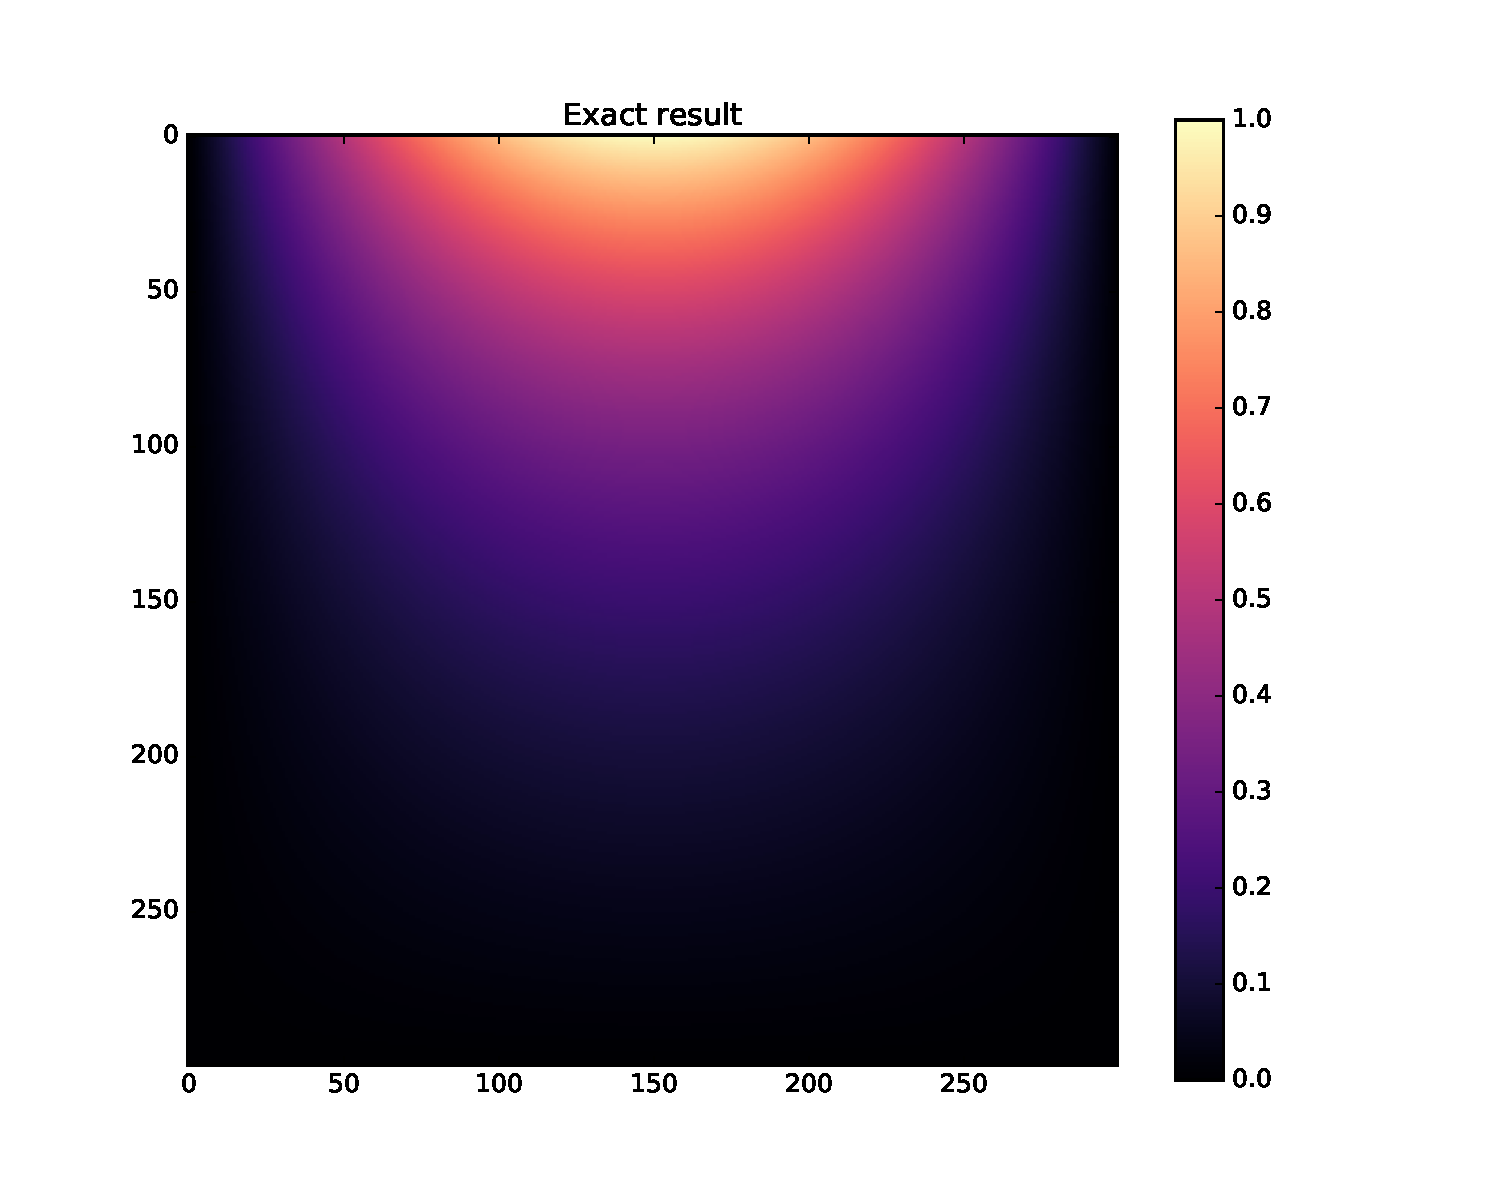
\includegraphics[width=1.1\linewidth]{sin300_exact.pdf}
	\caption{More realistic view of CPU and RAM.}
	\label{fig:sin-analytic}
	\end{figure}

Figure~\ref{fig:sin-result} shows the output of the solver program in single-threaded mode when given the $\sin(x)$ along one side
potential, plotted with the Python library matplotlib. The configuration has a grid size of 300 by 300. It matches very well with the analytical result, which
is
$$\frac{\sinh(y \pi / n)}{\sinh(\pi)} \sin(x \pi / n),$$
and is shown plotted in a similar way in figure~\ref{fig:sin-analytic}. The difference between the calculated result and the
analytical result is shown in figure~\ref{fig:sin-difference}. The values shown in the difference map are small compared
to the values in the result in all locations except the corners at the top, where the simulation does diverge somewhat, 
but never reaches values which are hugely divergence from the analytical result. Using the root-mean-square error statistic
described earlier, we have calculated that the RMS error in this simulation to be SOME NUMBER.


	\begin{figure}[h]
	\centering
	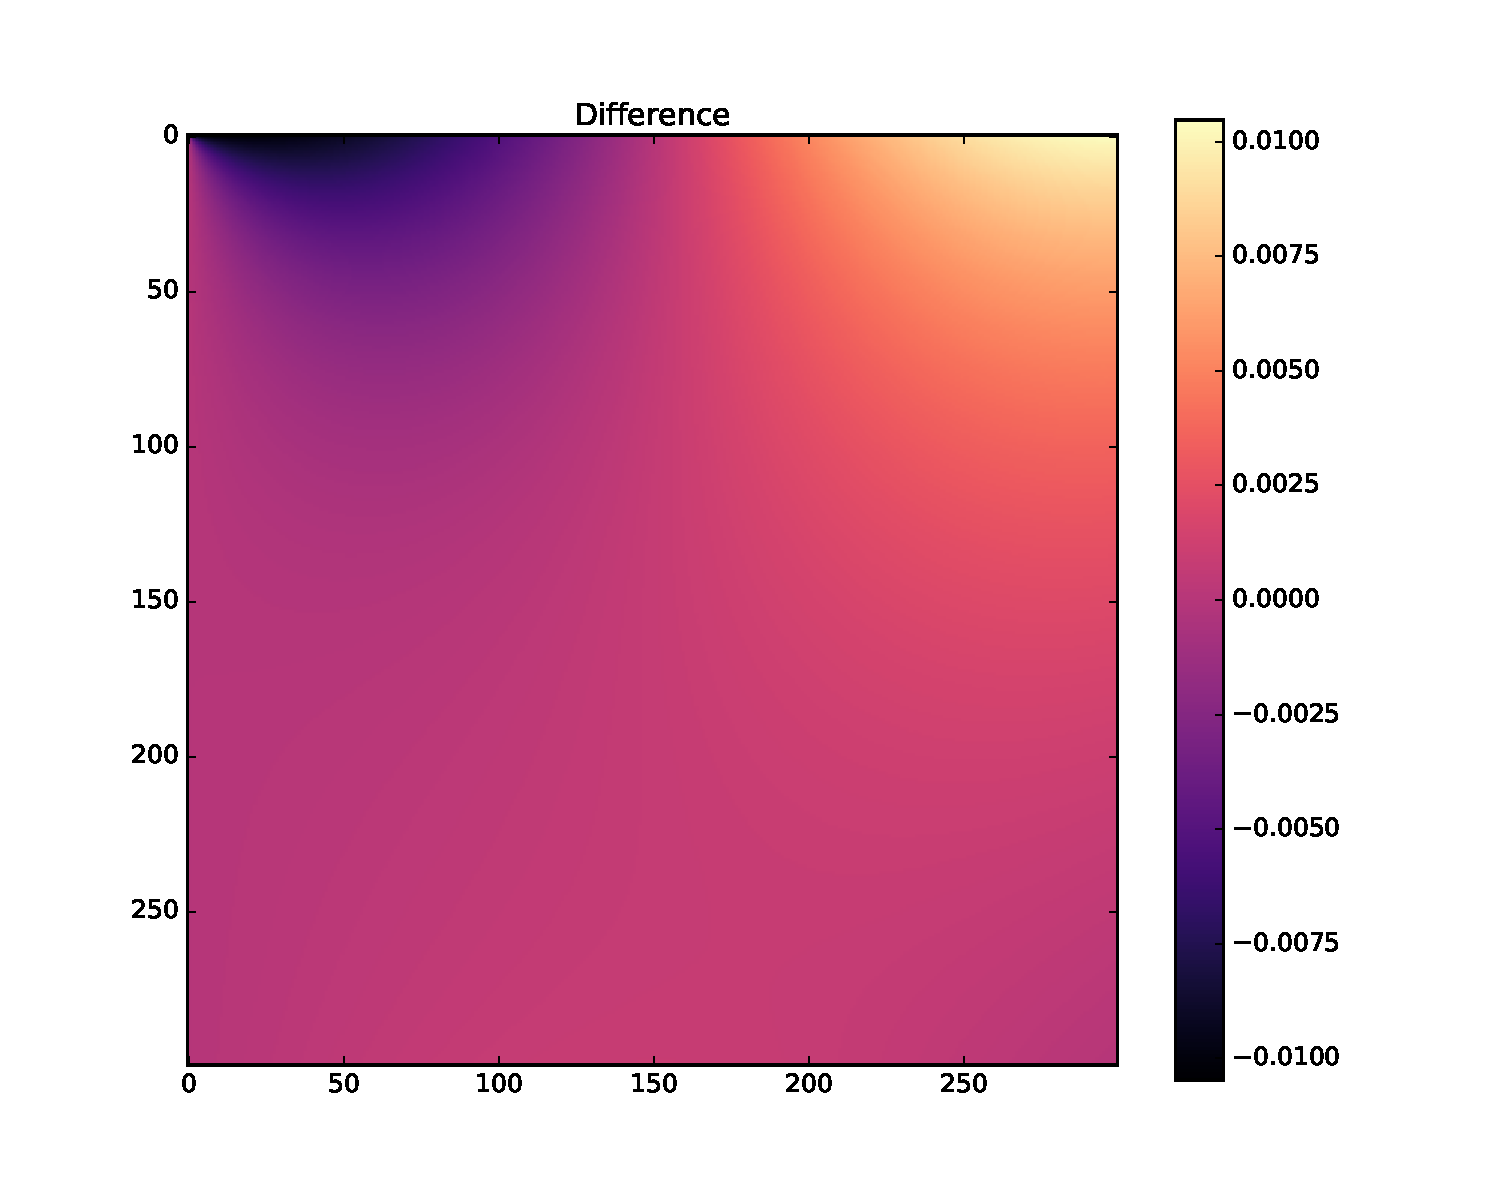
\includegraphics[width=1.1\linewidth]{sin300_diff.pdf}
	\caption{More realistic view of CPU and RAM.}
	\label{fig:sin-difference}
	\end{figure}

\subsection{Fitting to a $1/r^2$ Dipole Potential}

The dipole configuration had a grid size of 400 by 400, with all walls given a Dirichlet boundary condition
of zero. Two charges were placed near the center 10 cells apart with an arbitrary but equal and opposite charge.
The result of this simulation is shown in figure~\ref{fig:dipole-cont}, with the addition of constant-potential
contour lines. The simulation shows two opposite charges which near perfectly mirror each other. The vertical
line in the center represents a constant potential contour with a value of zero, which is expected from an
electric dipole. This is another excellent verifier that the simulation is producing correct results.

\begin{figure}[h]
	\centering
	\center
	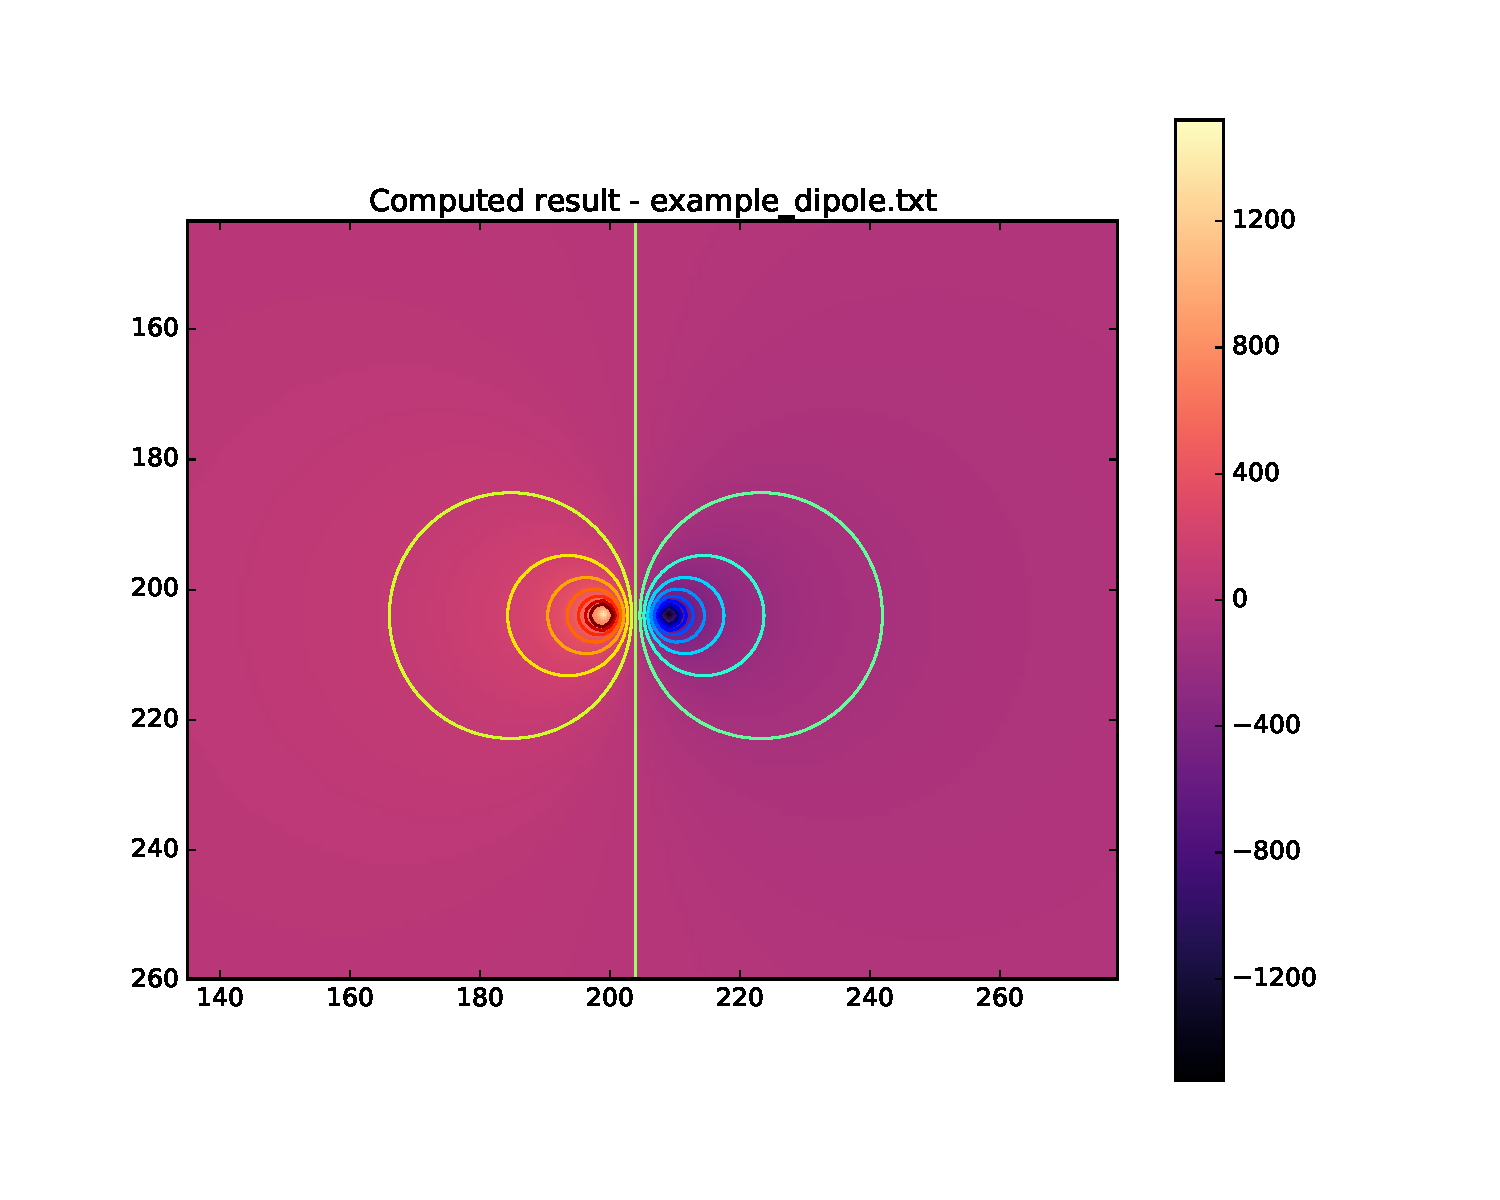
\includegraphics[width=1.1\linewidth]{dipole_contours.pdf}
	\caption{Fitting a $1/r^2$ curve to the calculated dipole potential.} \label{fig:dipole-cont}
	\end{figure}

The potential was then measured at locations increasing in distance from the dipole in an arbitrary direction.
These data were then plotted using gnuplot, and a line of the form $y(x) = A + B / (r-r_0)^2$ was fit to the
data, which is shown in figure~\ref{fig:dipole-fit} The fit is excellent, confirming that the program had properly simulated an electric dipole. The error
bars on the data points come from the difference between successive iterations at the end of the simulation of
the dipole. They are very small, but non-zero.



	\begin{figure}[h]
	\centering
	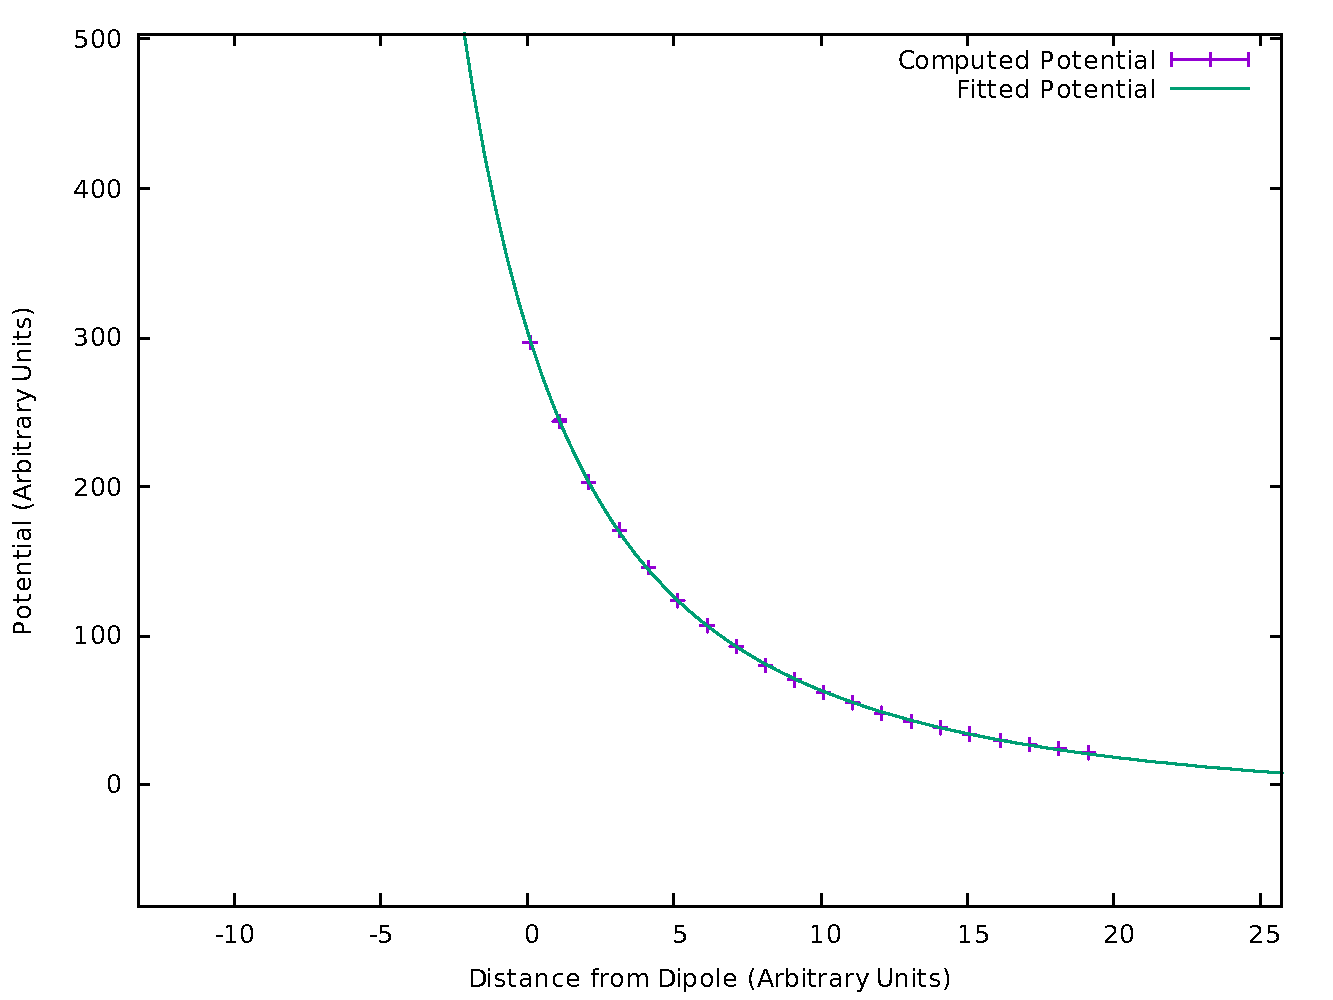
\includegraphics[width=\linewidth]{dipole_fit.pdf}
	\caption{Fitting a $1/r^2$ curve to the calculated dipole potential.} \label{fig:dipole-fit}
	\end{figure}

The dipole is an example which lends itself to presenting another feature of the solver program. If passed the
$\texttt{-V}$ option, it will take the negative gradient of the result and plot that as a vector field. This has
the effect of plotting the electric field of the result of the simulation, which for the dipole is shown in
figure~\ref{fig:dipole-field}.

	\begin{figure}[h]
	\centering
	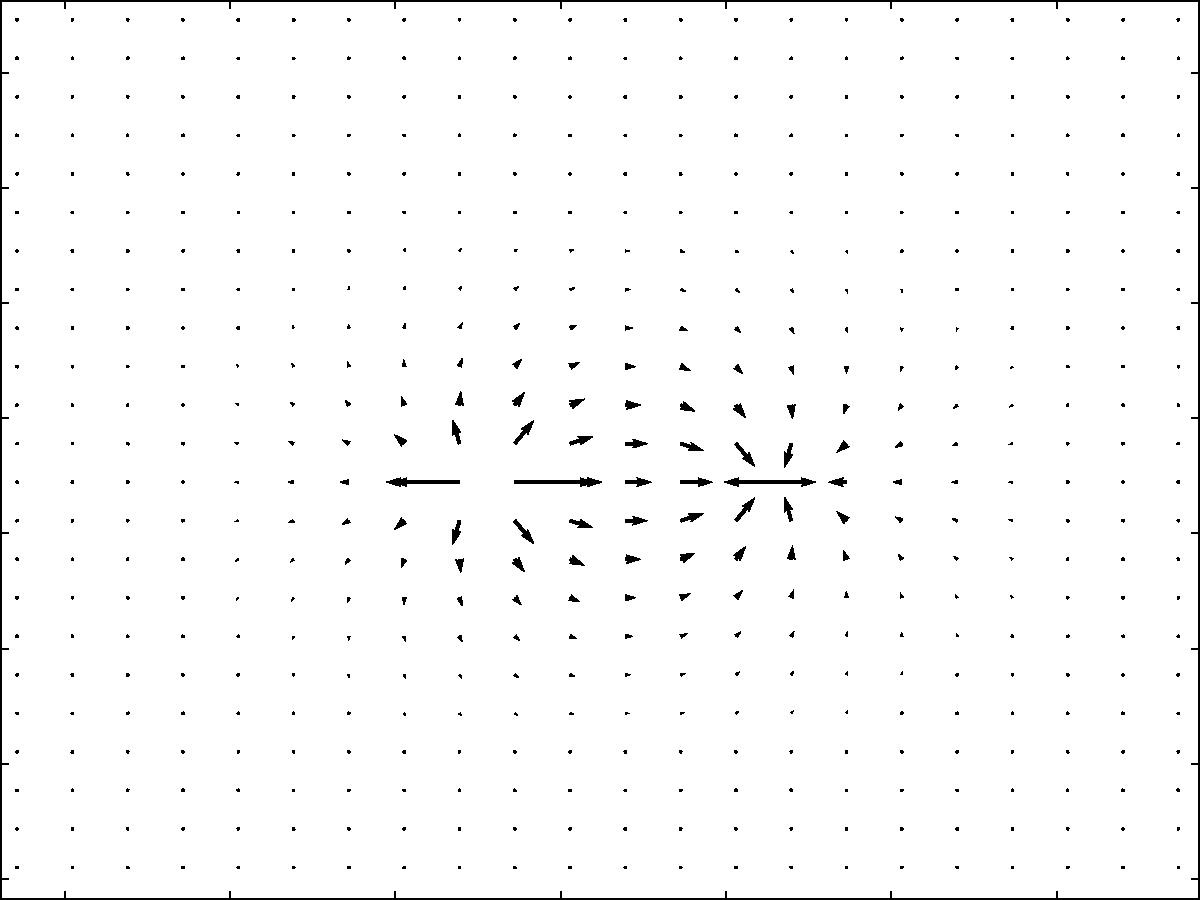
\includegraphics[width=0.7\linewidth]{dipole_field.pdf}
	\caption{Fitting a $1/r^2$ curve to the calculated dipole potential.} \label{fig:dipole-field}
	\end{figure}


\subsection{Performance}


Figure~\ref{fig:perf-sizes} shows the performance in iterations per second for a varying grid size for given
configuration, in this case the $\sin(x)$ along a wall potential. The performance tests were run square grids
of size 50 by 50, 300 by 300, and 1000 by 1000. For each grid size, 4 different simulation options were given:
single-threaded non-SIMD, single-threaded SIMD, multi-threaded with 4 threads non-SIMD, and multi-threaded
with 4 threads and SIMD.


\begin{figure}[h]
	\centering
	\pgfplotstableread{
		0 35 10    8 10     134 10    666 1000
		1 35 10    1461 15     134 10    666 1000
		2 132.845 1.36    127.085 3.45     297.9 23.13    222.8 26.7
	}\dataset
	\begin{tikzpicture}
    \begin{axis}[
    	xticklabels = {
    		sin50,
    	    sin300,
    	    sin1000,
    	},
        xtick=data,
        major x tick style = transparent,
        width  = 0.85*\textwidth,
        height = 8cm,
        major x tick style = transparent,
        ybar=2*\pgflinewidth,
        bar width=14pt,
        ymajorgrids = true,
        ylabel = {Run time speed (iters/sec)},
        xtick = data,
        major x tick style = {opacity=0},
        minor x tick num = 1,
        minor tick length=2ex,
        ymin=0,
        legend cell align=left,
		legend style={
	        anchor=south east,
	        column sep=1ex
	    },
        ]

\addplot[draw=black,fill=black!20, error bars/.cd, y dir=both, y explicit] table[x index=0,y index=1, y error index=2] \dataset; %Data1
\addplot[draw=black,fill=black!40, error bars/.cd, y dir=both, y explicit] table[x index=0,y index=3, y error index=4] \dataset; %Data2
\addplot[draw=black,fill=black!60, error bars/.cd, y dir=both, y explicit] table[x index=0,y index=5, y error index=6] \dataset; %Data3
\addplot[draw=black,fill=black!60, error bars/.cd, y dir=both, y explicit] table[x index=0,y index=7, y error index=8] \dataset; %Data3

	\legend{Single Threaded SIMD, Single Threaded, Multithreaded (4 threads), Multithreaded (4 threads) SIMD}
\end{axis}
\end{tikzpicture}
\caption{Different grid sizes for the $\sin(x)$ configuration, and their performance characteristics.}
\label{fig:perf-sizes}
\end{figure}

%		\addplot[ybar,fill=green,mark=none] coordinates {(0,   1513.05)};
% \addplot[ybar,fill=blue,mark=none] coordinates {(0,   1459.24)};
% \addplot[ybar,fill=red] coordinates {(0,   3174.49)};
% \addplot[ybar,fill=orange] coordinates {(0,   2354.03)};

	% \addplot[ybar,fill=green,mark=none] coordinates {(1,   1513.05)};
	% \addplot[ybar,fill=blue,mark=none] coordinates {(1,   1459.24)};
	% \addplot[ybar,fill=red] coordinates {(1,   3174.49)};
	% \addplot[ybar,fill=orange] coordinates {(1,   2354.03)};

	% \addplot[ybar,fill=green,mark=none] coordinates {(2,   1513.05)};
	% \addplot[ybar,fill=blue,mark=none] coordinates {(2,   1459.24)};
	% \addplot[ybar,fill=red] coordinates {(2,   3174.49)};
	% \addplot[ybar,fill=orange] coordinates {(2,   2354.03)};












Figure~\ref{fig:perf-numthreads} shows the performance in iterations per second of the solver when run
with the $\sin(x)$ potential with a grid size of 300 by 300. This was done on computer B, and so was done
only in non-SIMD mode. The results show a significant improvement in performance when using multiple threads
compared to the single threaded case. One may na\"{i}vely have expected the performance to scale linearly
with the number of threads; however, this would be very unlikely. As the number of threads goes up, the amount
of work that can be done in parallel would seem to scale with the number of threads, until one considers processor cache effects (specifically
cache coherency and cache size limitations). This is seen in the case of 4 threads, as it is not 4 times as fast as
the single threaded case, only about 3.2 times as fast. Increasing the number of threads quickly starts giving diminishing
returns, as the 8 threads case is now only slightly better than the 4 threads case. Recall that computer B, on which these
tests are run, has 4 cores with 2 threads each, totally 8 possible threads running in parallel. After the 8 threads case,
we start to see a drop in performance; the 16 and 32 threads case are worse than the 8 threads case. This is because
the machine cannot run more than 8 threads in parallel, so in order to have 16 threads it must rely on the scheduling
of the operating system in order to get work done. In a case of many threads, each doing heave computation and memory accesses
(as is the case here), it does not usually help to increase the number of threads beyond what the machine can handle,
as is shown here.

\begin{figure}[h]
	\centering
	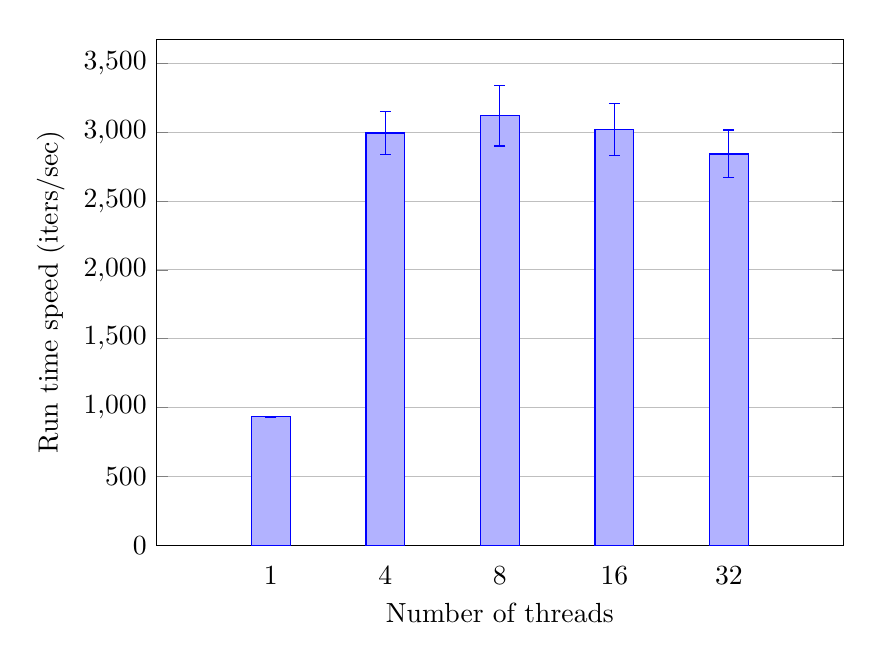
\begin{tikzpicture}
    \begin{axis}[
        xtick=data,
        symbolic x coords={1, 4, 8, 16, 32},
        major x tick style = transparent,
        width  = 0.85*\textwidth,
        height = 8cm,
        major x tick style = transparent,
        ybar=2*\pgflinewidth,
        bar width=14pt,
        ymajorgrids = true,
        ylabel = {Run time speed (iters/sec)},
        xlabel = {Number of threads},
        xtick = data,
        scaled y ticks = false,
        enlarge x limits=0.25,
        ymin=0,
        legend cell align=left,
		legend style={
	        anchor=south east,
	        column sep=1ex
	    },
        ]
            \addplot+[error bars/.cd,
                       y dir=both, y explicit]
                    coordinates {
                    (1, 933.156)  +- (3.612, 3.612)
                    (4, 2994.42)  +- (157.1, 157.1)
                    (8, 3119.1)  +- (219, 219)
                    (16, 3020.6)  +- (190, 190)
                    (32, 2842)  +- (174, 174)
                    };
\end{axis}
\end{tikzpicture}
\caption{Performance results for a varying number of threads in non-SIMD mode. These
tests were done on computer B, using the $\sin(x)$ potential with a grid size of 300 by 300.}
\label{fig:perf-numthreads}
\end{figure}



Furthermore, figure~\ref{fig:err-numthreads} shows that it is disadventagous to run the simulation with
a large number of threads. The RMS error of the simulation compared to the analytical result increases
rapidly with the number of threads. This is also reflected in the result of the simulation, which is
noticably wrong in the case of 16 or higher threads. I believe this to be the result of the way the threads
are synchronized, or more accurately, how they are not. The threads run mostly in isolation, sharing the
grid and doing operations on it without waiting for other threads to complete any of their work. This means
that if one threads runs faster than the others, it may complete a different number of iterations than the other
threads in a given amount of time. This would result in some sections of the grid recieving more iterations
than others, which could have the effect of invalidating the simulation. The alternative method would be
to synchronize the threads, and have them wait for each thread to complete a given iteration before moving on
to the next one. Indeed, this was the original design of the system, and I found it to be so slow compared to
single threaded that I changed the design around to the less accurate but much faster design that is shown here.



\begin{figure}[h]
	\centering
	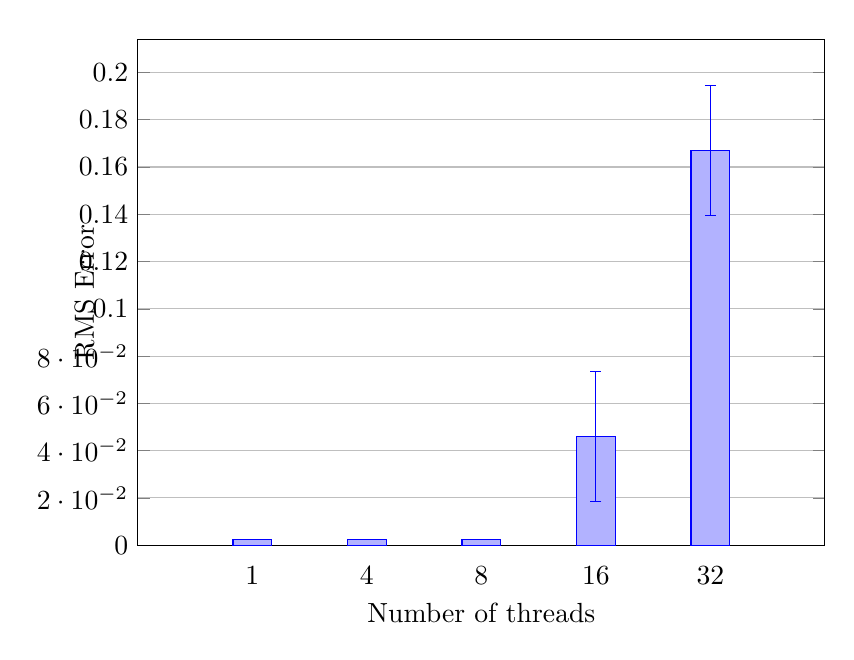
\begin{tikzpicture}
    \begin{axis}[
        xtick=data,
        symbolic x coords={1, 4, 8, 16, 32},
        major x tick style = transparent,
        width  = 0.85*\textwidth,
        height = 8cm,
        major x tick style = transparent,
        ybar=2*\pgflinewidth,
        bar width=14pt,
        ymajorgrids = true,
        ylabel = {RMS Error},
        xlabel = {Number of threads},
        xtick = data,
        y label style={at={(axis description cs:-0.05,.5)},rotate=0,anchor=south},
        enlarge x limits=0.25,
        try min ticks=10,
        ymin=0,
        legend cell align=left,
		legend style={
	        anchor=south east,
	        column sep=1ex
	    },
        ]
            \addplot+[error bars/.cd,
                       y dir=both, y explicit]
                    coordinates {
                    (1, .002544)  +- (0, 0)
                    (4, .002544)  +- (.000000027, .000000027)
                    (8, .002544)  +- (.0000000269, .0000000269)
                    (16, .046)  +- (.0274, .0274)
                    (32, .167)  +- (.0274, .0274)
                    };
\end{axis}
\end{tikzpicture}
\caption{Error results for a varying number of threads in non-SIMD mode. These
tests were done on computer B, using the $\sin(x)$ potential with a grid size of 300 by 300.}
\label{fig:err-numthreads}
\end{figure}



%32 ave: 0.166412 sq: 0.0277446 stddev: 0.00718529


\section{Conclusion}

This program correctly solves certain boundary value problems, enabling simulation
of complex electrostatics situations. It does this in an efficient manner by leveraging
proper programming languages and techniques and utilizing the basics of modern processor
design. There were numerous surprises found in developing this software and looking at
the resulting physics that it described.

\subsection{Correctness}

The most important aspect of this program is that is produces an accurate result, no
matter how fast it runs. I was able to use a problem for which I had an analytical
solution to confirm that the simulation was producing accurate results and found that
the results were of high quality for the single threaded and low number of threads
cases. Additionally, I was able to use the solver program to accurately calculate
that the electric potential from an electric dipole drops off as $1/r^2$, further
confirming the correctness of the program.


\subsection{Performance}

Since the simulation is correct, I was able to then turn my attention towards improving
the performance without reducing the accuracy of the simulation. Most of this was easy to
do without reducing accuracy, as it was simply transforming one valid implementation of
the code into another and measuring to ensure that my new implementation did in fact
cause an improvement. Most of this was done by improving cache locality and reducing
memory accesses. I have left out a lot of this process for brevity, however an overview
of it and the concepts used can be found in appendix~\ref{app:opt}.

The next significant performance gain attempt that I had made was the use of SIMD instructions.
I was hoping for a much more significant performance boost than I saw, which was rather
miniscule in reality. The only small improvement was not surprising in the single threaded
case because I knew that \texttt{gcc} utilizes SIMD when it can, but I did not expect to see
the manual SIMD instructions degrade the performance in the multi-threaded case. I speculate
that this is caused by my manual SIMD code being less cache friendly, which is okay in the
single threaded case and allowed a small performance improvement, but in the multithreaded case
the threads are all contending for limited cache space, so the additional memory usage slowed
them down.

The multithreading actually improved the performance significantly more than I expected it to.
I had predicted that the algorithm would be cache-bound due to the large amount of memory accesses
that it makes. This often results in insignificant performance improvements (or downright performance
degredation) when adding multiple threads to a single threaded program. Of course, the cardinal
rule of any scientific experiment (including attempting to optimize a program) is to measure and
compare results. Clearly the multi-threaded case is significantly better in performance, with a trade-off
in accuracy, which may certainly be acceptible.

\subsection{Future Work}

There is still a significant amount of optimization work that can be done on this program. A careful reading
of Intel optimization manuals would likely provide numerous ideas for how to further improve the code
for the program. The manual SIMD code could also be improved, either by utilizing more up-to-date instruction
sets or by improving the existing algorithm. The multithreaded code could also be improved, by allowing the threads
to communicate in a limited way in order to better synchronize their work to improve the quality of the result without
hopefully degrading the performance too drastically. An additional approach could be to use the multithreaded case for
a few hundred iterations before switching over to the single threaded version in order to smooth out and cleanup the
results. This would have a significant advantage for large simulations, as the multithreaded code could get the result
most of the way before letting the single threaded code produce an accurate result in a shorter amount of time than
if the single threaded code ran from the start.

Another significant way in which to improve the real world performance of the program is in addition to optimizing
the speed at which the program can calculate an iteration, to reduce the number of iterations required to
converge on a solution. Indeed, this is what the use of successive over-relaxation achieves, but there may be ways
to further improve this. One such method could be to improve the initial ``guess'' of zero everywhere by dividing
the grid into a much coarser grid and running a few iterations on that before returning to the full grid and completing
the simulation as before.

\begin{center}\rule{2cm}{0.4pt}\end{center}




\clearpage
\begin{appendices}
\section{Program Usage}

Compiling the engine (the C library) requires make and gcc (or clang, although clang is untested), and can
be done by simply invoking \texttt{make}. This will also create an executable file, \texttt{solve}. This
is a script that invokes the python example frontend so that it may be used.

For more details on using the python frontend or the C backend engine, see the man pages (reproduced on the
following pages). There are several example files, including \texttt{example\_sin.txt} and \texttt{example\_dipole.txt}.
For more details on writing configurations for a desired simulation or experiment, see the man pages.

The source code also contains a directory named \texttt{tests}, which contains python code to generate verifier data
files for the \texttt{example\_sin} configuration. Finally, all of the data written on in this document are present
in the source directory, under \texttt{results}. The source code for the C library is in \texttt{engine}, and the
source code for the python example frontend is under \texttt{frontend}. The source code and git revision history
is available at \url{http://github.com/dbittman/statics-solver}.

	\begin{singlespacing}
\begin{flushleft}
	SOLVE(1)
	\hfill User Commands \hfill
	SOLVE(1)
\end{flushleft}

\begin{tabbing}
\hspace{30pt}\=\hspace{30pt}\=\kill

\textbf{NAME}\\
\> solve - Solve Discreet Poisson Equation\\
\\
\textbf{SYNOPSIS}\\
	\> \texttt{solve [-V] [-m \textit{method}] [-v \textit{verification-data}] \textit{configuration-file}}\\
	\\
\textbf{DESCRIPTION}\\
\> Solve Poisson Equation given boundary conditions on a discreet grid. Capable of\\
\> solving physics problems that reduce to a boundary value problem. Operates on the\\
\> provided configuration file, producing a 2-D array describing the calculated potential.\\
\\
\> \texttt{\textbf{-V}} \\
\> \> Produce a vector plot, where the vectors are the negative gradient of the potential.\\
\\
	\> \texttt{\textbf{-m} \textit{method}} \\
	\> \> Use method \textit{method} when solving. Current supported values are \texttt{jacobi} for\\
	\> \> Jacobi Iteration, and \texttt{sor} for Successive Over-Relaxation.\\
\\
	\> \texttt{\textbf{-v} \textit{verification-data}} \\
	\> \> Use the data file \textit{verification-data} to compare with the generated potential. The \\
	\> \> format for this file must be that of the python library pickle serializing a 2-D array.\\
\\
\textbf{CONFIGURATION}\\
\> The configuration file format is specified by a series of commands on lines. A single line\\
\> can contain at most one command. A command must be contained within one line.\\
\> Comments begin with a \#, and comment out the rest of that line. Valid commands are\\
\> as follows, where italics indicates something to be replaced by one token:\\
\\
	\> \texttt{gridsize \textit{size}}\\
	\> \> Set the size of the grid. The grid is always a square, and this command \textbf{must}\\
	\> \> come before any other.\\
	\\
	\> \texttt{cell \textit{coords} initial \textit{value}}\\
	\> \> Specify initial value of a cell inside the grid. Analogous to a point charge.\\
	\\
	\> \texttt{dirichlet \textit{coords} \textit{coords} = \textit{value}}\\
	\> \> Specify a diriclet boundary condition along the interpolated straight line from the\\
	\> \> first set of coordinates to the second with value \textit{value}.\\
\end{tabbing}
\begin{flushleft}
	statics-solver
	\hfill March 2016 \hfill
	SOLVE(1)
\end{flushleft}
\clearpage
\begin{flushleft}
	SOLVE(1)
	\hfill User Commands \hfill
	SOLVE(1)
\end{flushleft}

\begin{tabbing}
\hspace{30pt}\=\hspace{30pt}\=\kill
	\> \texttt{neumann \textit{coords} \textit{coords} \textit{direction} = \textit{value}}\\
	\> \> Specify a diriclet boundary condition along the interpolated straight line from the\\
	\> \> first set of coordinates to the second with value \textit{value} across the boundary of the\\
	\> \> cells specified by \textit{direction}, which may be one of \texttt{left, up, right, down}.\\
	\\
	\> The values of \texttt{\textit{coords, size, direction}} must all be one token, that is,\\
	\> they may not contain any whitespace. The contents of \texttt{\textit{value}} and \texttt{\textit{coords}} are\\
	\> as follows:\\
	\\
	\> \texttt{\textit{value}} is an \texttt{expression}.\\
	\\
	\> \texttt{\textit{coords}} is an \texttt{expression} followed by a comma, followed by an \texttt{expression}.\\
	\\
	An \texttt{expression} is a valid python expression, with access to the python math library, the\\
	current grid class, and the current position in the grid as specified by \texttt{x} and \texttt{y}. For \\
	example, \texttt{math.sin(x*math.pi/grid.len)} is a valid \texttt{expression}.\\
	\\
	\textbf{AUTHOR}\\
	\> Written by Daniel Bittman (\texttt{danielbittman1@gmail.com}). Please submit any bug\\
	\> reports to this email address.\\
	\\
	\textbf{COPYRIGHT}\\
	\> Copyright\copyright Daniel Bittman. License MIT software license. This is free software, and\\
	\> is provided with NO WARRANTY.\\
	\\

\end{tabbing}
\begin{flushleft}
	statics-solver
	\hfill March 2016 \hfill
	SOLVE(1)
\end{flushleft}


\begin{flushleft}
	SOLVER(3)
	\hfill Libraries \hfill
	SOLVER(3)
\end{flushleft}

\begin{tabbing}
\hspace{30pt}\=\hspace{30pt}\=\kill

\textbf{NAME}\\
\> solver - Library to solve Discreet Poisson Equation\\
\\
\textbf{SYNOPSIS}\\
	\> \texttt{solver.h}\\
	\> \> \texttt{SOLVE\_METHOD\_JACOBI}\\
	\> \> \texttt{SOLVE\_METHOD\_SOR}\\
	\> \texttt{double \textbf{solve}(struct grid *grid, int method);}\\
	\> \texttt{void \textbf{init\_grid}(struct grid *grid);}\\
	\> \texttt{struct grid \{}\\
	\> \> \texttt{int len;}\\
	\> \> \texttt{int iters;}\\
	\> \> \texttt{float **values;}\\
	\> \> \texttt{float **value\_prevs;}\\
	\> \> \texttt{float **initials;}\\
	\> \> \texttt{uint8\_t **dirichlet\_presents;}\\
	\> \> \texttt{float **dirichlets;}\\
	\> \> \texttt{uint8\_t **neumann\_presents;}\\
	\> \> \texttt{float **neumanns[4];}\\
	\>\texttt{\};}\\
\\
\textbf{DESCRIPTION}\\
\> This library provides fast solving of a 2-D discreet boundary value problem using the\\
	\> Poisson equation. The full process is to define a \texttt{struct grid}, and set its \texttt{len} field. Then\\
	\> call \texttt{init\_grid} on the grid to initialize the 2-D contiguous arrays. After that, call \texttt{solve}\\
	\> and pass it the grid and a method, either \texttt{SOLVE\_METHOD\_JACOBI} or \texttt{SOLVE\_METHOD\_SOR}.\\
	\\
	\> The \texttt{solve} function will return when complete, returning back a value describing how\\
	\> confident it is in its result (values closer to zero are better). The \texttt{iters} field in the grid\\
	\> will have been updated to indicate how many iterations the program took. The \texttt{values}\\
	\> field points to a 2-D array of size \texttt{len} by \texttt{len} containing the solution.\\
	\\
	\textbf{AUTHOR}\\
	\> Written by Daniel Bittman (\texttt{danielbittman1@gmail.com}). Please submit any bug\\
	\> reports to this email address.\\
	\\
	\textbf{COPYRIGHT}\\
	\> Copyright\copyright Daniel Bittman. License MIT software license. This is free software, and\\
	\> is provided with NO WARRANTY.\\
	\\

\end{tabbing}
\begin{flushleft}
	statics-solver
	\hfill March 2016 \hfill
	SOLVER(3)
\end{flushleft}


	\end{singlespacing}
\clearpage

\section{Computer Program Optimization} \label{app:opt}

When optimizing a program, there is an important cardinal rule to follow which at times
is easy to forget in the face of increasingly interesting and complex minor optimizations
designed to squeeze every bit of performance out of your computer. Unfortunately, due
to the complexity of modern computer hardware, it is
very difficult to predict if a given micro-optimization will actually be benificial or
not. For this reason, the most important rule when taking a working program and making it
fast is\footnote{besides \textit{don't break it}, of course. An incorrect program is worthless, no matter
how fast it is.} \textit{benchmark everything}.

The field of program optimization is huge. There is a small number of people who, for
a given platform, are really \textit{good} at optimization. There is an even smaller number
who are truly experts. I do not fit into either of these categories. For this reason, the program
that I have written here is \textit{decently} optimized. I believe that the maximum throughput
is not orders of magnitude better than what I have achieved, however, there is still a lot of work
that can be done (including a potentially significant optimization that I have neglected, and will talk
about later).

%%%%%%%%%%%%%%%%%%%%%%%%%%%%%%%%%%%%%%%%%% ACTUALLY TALK ABOUT THAT ************************

\subsection{Freebies}

There are some optimizations which can be used in high confidence and are also very easy to do.
The first, and most obvious, is to use a fast language. While writing in \texttt{C} may be a chore
compared to writing in python, the resulting code will be much faster. This is the reason behind the
organization of this program: the frontend (which has no performance requirements) is written in
python because parsing the configuration file is much easier. The backend needs to be fast, so it
is implemented in \texttt{C}.

A quick and rough experiement can easily convince you that this is true (remember how I said to
benchmark everything?). Credit to my friend Chris Milke for doing this test. Write the following
code in both python and in C: initialize a variable to zero. Then loop from zero to some large
number (we used 123,456,789), and add that iteration to the variable. After the loop, print the
variable. The resultant python program took 14.25 seconds to run on my computer, but the C code
completed \textit{instantaneously}. Why is python slower than C in general? Because python is
an interpreted language. The code that you write is read by another program and executed by
that program. In contrast, C code must be compiled into machine code. This is then run directly
on the processor, which cuts out the middle-man of the interpreter.

When using C, there are some more things that you can get for free: compiler optimizations. When
compiling a C program, the command looks something like this: \texttt{gcc -Wall -Wextra foo.c}\footnote{as an aside, you should \textbf{always} compile with -Wall and -Wextra, and eliminate all warnings from your program.
Warnings are warnings for a reason, and should rarely be ignored.}. This will
result in a compiled C program (a binary file, containing the machine code), but it will be
unoptimized. There are reasons why one may want an unoptimized binary (they are typically
easier to debug, for example), but generally when you compile your program for actual usage
you will want to optimize it. An aggressive optimization compilation command may look something
like: \texttt{gcc -Wall -Wextra -O3 -ffast-math -mavx}, as a start. The main flag here is \texttt{-O3}, which
enables almost every optimization that gcc can do.

Going back to the example from earlier, the optimized version of the C program completed instantly, but
the unoptimized version took 0.33 seconds. The unoptimized version is still 43 times faster than the
python code, but what was the optimizing compiler doing to make it so much faster with \texttt{-O3} on?
Part of optimizing is understanding why something is faster, so lets look at the assembly code. On \textsc{unix},
this can be done with the objdump command. Table \ref{table:assem-1} shows the annotated assembly from
the function \texttt{main}. If you don't know x86\_64 assembly language, you will at least notice that the
optimized version is much shorter. If you do know how to read the assembly, you'll notice that the unoptimized
version is doing almost literally what the C code says to do: set a variable to zero, and iterate from zero to
a big number, adding that iteration to the variable, and finally printing the variable. The optimized code just prints a large number -- which happens to be the result of the sum.

\begin{table}[h]
	\centering
\begin{tabular}{l | l}
	\hline
	\textbf{Unoptimized} & \textbf{Optimized}\\
	\hline
	\texttt{mov [rbp-0x10], 0x0}	&\texttt{movabs rsi,0x1b131147ee6b52} \\
	\texttt{jmp .loop\_end			}	&\texttt{mov edi,0x400594} \\
	\texttt{.loop\_top:                } &\texttt{xor eax,eax   } \\
	\texttt{mov rax, [rbp-0x10]				}	&\texttt{jmp 4003c0 <printf@plt>}\\
	\texttt{add [rbp-0x8], rax				}	&\texttt{	} \\
	\texttt{add [rbp-0x10], 0x1				}	&\texttt{ }\\	
	\texttt{.loop\_end:                       } &\texttt{} \\
	\texttt{cmp [rbp-0x10],0x75bcd14} &\texttt{} \\
	\texttt{jle loop\_top} &\texttt{} \\
	\texttt{mov rsi,[rbp-0x8]} &\texttt{} \\
	\texttt{mov edi, 0x4005b4} &\texttt{} \\
	\texttt{mov eax, 0} &\texttt{} \\
	\texttt{call 4003c0 <printf@plt>} &\texttt{} \\
\end{tabular}
	\caption{Unoptimzed and optimized assembly from the sum-a-lot-of-numbers example.}
	\label{table:assem-1}
\end{table}

This is just a simple example, but a good C compiler can drastically improve the performance of a
program. Here, it made a program that took a third of a second (which is already drastically faster than
the interpreted python version!) finish instantly.

\subsection{A Model of Processor Design}



\begin{figure}[h]
\begin{subfigure}{0.4\textwidth}
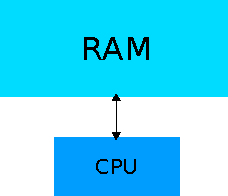
\includegraphics[width=\linewidth]{ram-cpu-simple.pdf}
\caption{Simplistic view of CPU and RAM.} \label{fig:1a}
\end{subfigure}
\hfill
\begin{subfigure}{0.4\textwidth}
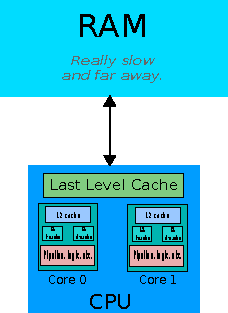
\includegraphics[width=\linewidth]{ram-cpu-complex.pdf}
\caption{More realistic view of CPU and RAM.} \label{fig:1b}
\end{subfigure}
\label{fig:cpu-and-ram}
\caption{View of programming that programmers like to have (a), versus the the more realistic
and complicated view.}
\end{figure}


\subsection{Structure of Arrays}

\subsection{Multithreading}

\subsection{Vectorization}
\subsubsection{Branch Reduction}






\section{Program Implementation}
\label{app:des}
The procedure of the program implementation was completed in multiple phases designed to section off
the different aspects of the designing the program into more managable pieces while allowing me to ensure
that each transformation that I made to the program was one such that the program did not lose functionality
or correctness at any stage. Before writing any code, I had a general understanding of the math behind the
algorithm. This did not mean, however, that I was completely sure that the implementation would be correct,
thus necessitating testing. As discussed previously, I designed several test cases for which I knew what the
correct solution was.

%\subsection{Designing for Correctness}
The first iteration of the program was a simplified and not optimal version written entirely
in C in order for me to confirm the correctness of my approach. This version made no attempts to
be fast and had the boundary conditions and grid parameters hard-coded into it. I implemented
Jacobi iteration and SOR, both of which arrived at the correct result for the $\sin(x)$ potential
along a wall.

I next turned my attention to the question of how to interface with the program. Hard-coded boundary conditions
are not desireable, and I quickly found it bothersome to have to modify the code in order to change the conditions
to further test the program. I decided to use a python script to process a configuration file and then call into a
C library which would do the heavy lifting. This is a common approach when dealing with processor intensive simulations
because it allows the speed of C while allowing for the ease of python scripting in order to setup the simulation and
process the results. This necessitated defining a structure in C and a class in python which both contained the same
data in a layout that both C and python could agree upon. This ended up being not too complicated, except for the problem
that python would not allow me to define the memory layouts for the actual grid. To solve this problem, I had the C library
export another symbol which would initialize the data structures contained within the grid structure.

The python code was written to act as a parser for a configuration file and evaluate the result of calling the solver library.
Parsing the configuration file was not complicated, so that code was all written without external libraries. Evalutating the
returned data was done with a combination of the \texttt{numpy} and \texttt{matplotlib} python packages, allowing me to process
and display the results.

One this interface was defined and written, I turned back to the C code to improve the performance. The biggest performance increase
was seen by changing the data layouts to be a contiguous block of memory. Previously while making sure my understanding of the math was
correct, I had simply defined the layout of the cells of the grid to be an array of arrays (since it is 2 dimensional), but not necessarily
contiguous. After changing the allocation sceme, the performance improved dramatically. The second most significant improvement came from
changing the C code from an array-of-structures style data layout to a structure-of-arrays layout, as was discussed earlier. This resulted in
another significant performance boost.

After fixing up the general algorithms, I turned to a basic implementation of multithreaded. This took several iterations to get right. The threads
were each given a section of the array to operate on and they shared a global floating point value in order to determine if the simulation is stable, much like before.
Unlike before, this variables now needed to be atomic in order to avoid loss of data, as discussed previously. This slowed down the simulation
drastically because atomically symchronizing a floating point variable is extremely slow. I then changed the code so that each thread would individually keep
track of the stability of their own section of the grid, and when all of them agreed that the simulation was stable, they would complete. This significantly improved
the multithreaded performance, causing it to beat the single-threaded code.

\subsection{SIMD Implementation}
There were two use of SIMD inside the solver, each for doing one iteration of a given cell under one of two situations: with a Neumann boundary conditon, and
without. In the case of a non-Neumann influenced cell, the cell is calculated as a sum of its nearest neighbors along with its initial value scaled by a
factor of the inverse of the grid size. For successive over-relaxation, the code for an individual cells is shown in Listing~\ref{lst:normal}, and an abridged
SIMD version is shown in Listing~\ref{lst:simd-normal}.

\vspace{5mm}

\begin{minipage}{\linewidth}
\begin{lstlisting}[frame=single,label=lst:normal,caption={Iteration code (simplified) for a single cell. Also notice that this code uses structure-of-arrays data layout.}]
float value = grid->values[x][y+1];
value += grid->values[x][y-1];
value += grid->values[x-1][y];
value += grid->values[x+1][y];
value += params->h * grid->initials[x][y];
value *= params->omega / 4.;
grid->values[x][y]=value+(1.f-params->omega)*grid->values[x][y];
\end{lstlisting}
\end{minipage}

\begin{minipage}{\linewidth}
\begin{lstlisting}[frame=single,label=lst:simd-normal,caption={SIMD version of iteration code for a single cell. The loading of the initial vector is not shown for simplicity.}]
__m256 scal = _mm256_set1_ps(params->prefix2);
__m256 res = _mm256_mul_ps(v1, scal);
grid->values[x][y] = sum8(res);
\end{lstlisting}
\end{minipage}

The function calls beginning with \texttt{\_mm} are the SIMD instructions written in function form for C code. In this listing, \texttt{v1} is a vector that contains
the nearest neighbor values along with a scaled version of \texttt{grid->initials[x][y]} and the cell's previous value. In the second line, each of these elements is
multiplied by \texttt{scal}, much like multiplying a mathematical vector by a scaler value. The elements of the vector are then summed in the \texttt{sum8} function,
and the result of this is stored. The two listings are equivalent. The details of the \texttt{sum8} function and how the initial vector \texttt{v1} is loaded are
omitted here for brevity, but can be found in the source code.

The SIMD code that calculates Neumann boundary conditions is both more complicated and was not used in this thesis, so I will not discuss it in detail, except for one
particularly interesting aspect of it which is a common pattern when writing SIMD code. As discussed previously, it is important to avoid branching in code to improve
performance. The calculation for the Neumann boundary conditions involves testing a condition and throwing away a calculation depending on the result. Instead of
using \texttt{if} statements, we can instead always do all of the calculations, and then at the end select the ones that we want. This is akin to transforming the
code,
\begin{addmargin}[4em]{2em}% 1em left, 2em right
\begin{singlespace}
\texttt{uint32\_t x[2] = \{123, 456\};}\\
\texttt{uint32\_t result[2] = \{0, 0\};}\\
\texttt{if(condition1) result[0] = x[0];}\\
\texttt{if(condition2) result[1] = x[1];}\\
\end{singlespace}
\end{addmargin}
into,
\begin{addmargin}[4em]{2em}% 1em left, 2em right
\begin{singlespace}
\texttt{uint32\_t x[2] = \{123, 456\};}\\
\texttt{uint32\_t result[2] = \{0, 0\};}\\
\texttt{result[0] = x[0] \& mask1;}\\
\texttt{result[1] = x[1] \& mask2;}\\
\end{singlespace}
\end{addmargin}
where \texttt{mask1} and \texttt{mask2} are used to select which values to propegate forward in the calculation. The Intel SIMD instructions have a method to
create such masks easily based on a condition (but they do it in a way that does not involve branching). Because in SIMD doing a single multiplication and doing
four are no different in cost, this takes the approach of avoid branching by doing all of the calculations even though some are optional and then selecting the
ones that are wanted at the end.
In the SIMD code for the Neumann boundary conditions,
I use this technique.


\end{appendices}

\clearpage

\section*{Software Used}

\begin{enumerate}
	\item \texttt{gnuplot}. \url{http://www.gnuplot.info}
	\item \texttt{gcc}, and associated development toolchain. \url{http://gcc.gnu.org}, \url{https://www.gnu.org/software/binutils}, etc.
	\item \texttt{python 3}. \url{https://www.python.org}, including packages:
		\begin{enumerate}
			\item \texttt{matplotlib}
			\item \texttt{numpy}
			\item \texttt{ctypes}
			\item \texttt{pickle}
		\end{enumerate}
\end{enumerate}

\clearpage
\bibliographystyle{plain}
\bibliography{main}





\end{document}

